\documentclass[10pt]{article}
\usepackage[margin=0.88in]{geometry}
\usepackage{amsmath,amssymb,amsthm,mathtools}
\usepackage{graphicx}
\usepackage{microtype}
\usepackage[hidelinks,hypertexnames=false]{hyperref}

\newtheorem{theorem}{Theorem}
\newtheorem{corollary}{Corollary}
\newcommand{\R}{\mathbb R}
\newcommand{\Var}{\operatorname{Var}}

\title{The log-squared weight is sharp for the\
borderline logarithmic heavy tail}
\author{Candidate full answer to Example 2.28 of arXiv:0807.3112}
\date{13 August 2026}

\begin{document}
\maketitle

\noindent\textbf{Status.} Candidate full solution, pending expert review.
For the probability density in the source, the weight
$1+x^2\log^2(2+|x|)$ is exactly the asymptotic threshold for a weighted
Poincar\'e inequality.  In particular, the exponent $2$ cannot be lowered,
and no eventual $o(x^2\log^2 x)$ weight can replace it.

\medskip
\noindent\textbf{Source.} P.~Cattiaux, N.~Gozlan, A.~Guillin, and
C.~Roberto, \emph{Functional inequalities for heavy tails distributions and
application to isoperimetry}, arXiv:0807.3112, Example~2.28 on printed
page~12.\footnote{P.~Cattiaux, N.~Gozlan, A.~Guillin, and C.~Roberto,
arXiv:0807.3112 (2008).}  After proving
\[
 \Var_{\mu_q}(f)\le C_q\int |f'(x)|^2
       \bigl(1+x^2\log^2(2+|x|)\bigr)\,d\mu_q(x),
\]
the authors ask whether this weight is correct.  The same page recalls the
one-dimensional Muckenhoupt product that resolves the question.

\clearpage
\begin{center}
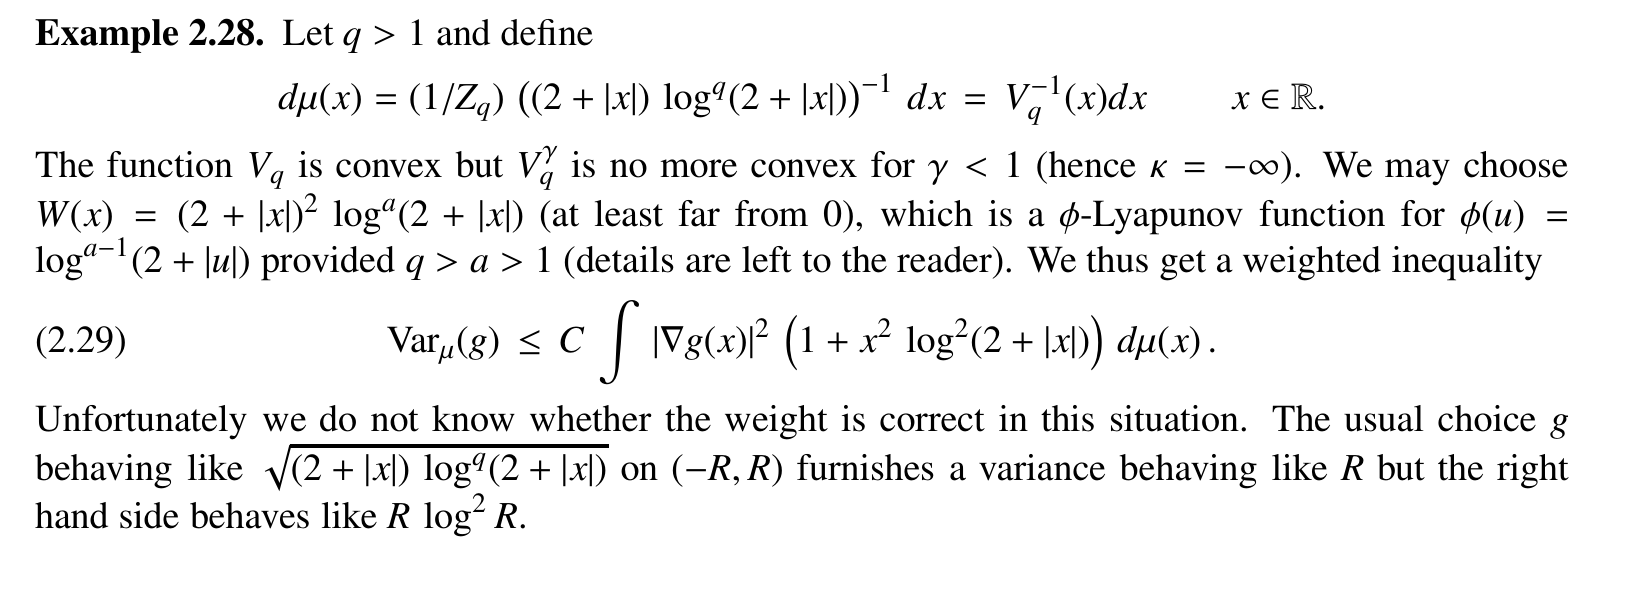
\includegraphics[width=0.96\textwidth]{figures/source_question_page12.png}

\small Figure 1: Example 2.28 and its open weight question in the archived
source PDF, printed page 12.
\end{center}

\section{Proof intuition}
In one dimension the issue is decided by a single tail--energy product:
the mass beyond $y$ is multiplied by the reciprocal weighted energy needed
to climb from the median to $y$.  For the present law these two factors
have opposite logarithmic powers, and their product stays bounded exactly
when the weight supplies two powers of $\log x$.  The Hardy criterion proves
sufficiency, while the associated one-sided equilibrium potentials are
matching test functions and therefore prove necessity.

\section{Exact criterion and answer}
Fix $q>1$, put $L(x)=\log(2+x)$ for $x\ge0$, and let
\[
 p_q(x)=\frac{1}{Z_q(2+|x|)\log^q(2+|x|)},\qquad
 d\mu_q(x)=p_q(x)\,dx.
\]
For a positive even continuous weight $W$, define
\begin{align*}
 T_q(y)&=\mu_q([y,\infty)),\\
 I_W(y)&=\int_0^y\frac{dx}{W(x)p_q(x)},\\
 B_W&=\sup_{y>0}T_q(y)I_W(y).
\end{align*}
Let $C_W$ be the least constant in
\begin{equation}
 \Var_{\mu_q}(f)\le C_W\int_{\R}|f'(x)|^2W(x)\,d\mu_q(x)       \tag{1}
\end{equation}
on the natural weighted Sobolev form domain.

\begin{theorem}[sharp criterion and threshold]\label{thm:main}
The weighted Poincar\'e inequality \emph{(1)} holds if and only if
$B_W<\infty$, and its best constant satisfies
\begin{equation}
 \frac12 B_W\le C_W\le4B_W.                                  \tag{2}
\end{equation}
Consequently:
\begin{enumerate}
\item for $W_\beta(x)=1+x^2\log^\beta(2+|x|)$,
      inequality \emph{(1)} holds if and only if $\beta\ge2$;
\item if $W(x)=o(x^2\log^2(2+x))$ as $x\to\infty$, then
      \emph{(1)} fails;
\item if $W(x)\ge c x^2\log^2(2+x)$ eventually for some $c>0$,
      then \emph{(1)} holds.
\end{enumerate}
Thus the source's log-squared weight is sharp in both the logarithmic-power
scale and the stronger eventual-comparison sense.
\end{theorem}

\section{Proof}
The upper inequality in (2) is the one-dimensional weighted Hardy theorem
used immediately before Example~2.28 in the source.  On $[0,\infty)$ it says
\[
 \int_0^\infty (f(x)-f(0))^2\,d\mu_q(x)
 \le4B_W\int_0^\infty |f'(x)|^2W(x)\,d\mu_q(x).
\]
Apply it on both half-lines and use
$\Var_{\mu_q}(f)\le\int(f-f(0))^2d\mu_q$ to obtain $C_W\le4B_W$.

For completeness, the converse and the obstruction can be seen directly.
For $y>0$ set
\[
 h_y(x)=
 \begin{cases}
 0,&x\le0,\\[2pt]
 \displaystyle\int_0^{\min\{x,y\}}\frac{ds}{W(s)p_q(s)},&x>0.
 \end{cases}
\]
Then
\[
 \int |h_y'|^2W\,d\mu_q=I_W(y),\qquad
 \int h_y^2\,d\mu_q\ge T_q(y)I_W(y)^2.                    \tag{3}
\]
Because $h_y$ is supported on a half-line of $\mu_q$-mass $1/2$,
Cauchy--Schwarz gives
\[
 \left(\int h_y\,d\mu_q\right)^2
 \le\frac12\int h_y^2\,d\mu_q,
\]
so $\Var_{\mu_q}(h_y)\ge\frac12\int h_y^2d\mu_q$.
Substitution in (1) and (3) yields
$C_W\ge\frac12T_q(y)I_W(y)$.  Taking the supremum proves the
lower inequality in (2).  Local smoothing at $0$ and $y$, while retaining
the two constant tails, gives the same conclusion in a smooth formulation
of (1).

It remains only to calculate the product.  The tail is exact:
\begin{equation}
 T_q(y)=\frac{1}{Z_q(q-1)}L(y)^{1-q}.                       \tag{4}
\end{equation}
For $W_\beta$,
\begin{align*}
 I_{W_\beta}(y)
 &=Z_q\int_0^y
   \frac{(2+x)L(x)^q}{1+x^2L(x)^\beta}\,dx\\
 &\sim Z_q\int^y\frac{L(x)^{q-\beta}}{x}\,dx.
                                                                    \tag{5}
\end{align*}
Hence, when $\beta<q+1$,
\begin{equation}
 I_{W_\beta}(y)\sim
 \frac{Z_q}{q-\beta+1}L(y)^{q-\beta+1},
\quad
 T_q(y)I_{W_\beta}(y)\sim
 \frac{L(y)^{2-\beta}}{(q-1)(q-\beta+1)}.                 \tag{6}
\end{equation}
At $\beta=q+1$, the integral in (5) is asymptotic to
$Z_q\log L(y)$; for $\beta>q+1$ it converges.  It follows that the product
is bounded exactly when $\beta\ge2$.  At the endpoint,
\[
 T_q(y)I_{W_2}(y)\longrightarrow\frac{1}{(q-1)^2},          \tag{7}
\]
which also displays the genuine criticality of the exponent $2$.

Finally suppose $W(x)=o(x^2L(x)^2)$.  Given $M>0$, for all sufficiently
large $x$,
\[
 \frac{1}{W(x)p_q(x)}
 \ge M Z_q\frac{(2+x)L(x)^{q-2}}{x^2}.
\]
After integration, (4) gives
$\liminf_{y\to\infty}T_q(y)I_W(y)\ge c_qM$.
As $M$ is arbitrary, $B_W=\infty$, proving failure.  Conversely, an eventual
lower bound by a positive multiple of $x^2L(x)^2$, together with positivity
and continuity on compact intervals, makes $B_W$ finite by comparison with
the endpoint case.  This completes the proof.

\section{What the source's test missed}
The source tests a truncated square root of the reciprocal density; for this
borderline tail it leaves a spurious factor $\log^2R$.  The correct
near-extremizers are the truncated Hardy potentials $h_y$ above.  For a
putative power $W_\beta$ their Rayleigh quotient obeys
\[
 \frac{\Var_{\mu_q}(h_y)}
      {\int |h_y'|^2W_\beta\,d\mu_q}
 \ge\frac12T_q(y)I_{W_\beta}(y)
 \asymp \log^{2-\beta}y,
\]
which diverges precisely below the exponent $2$.

\paragraph{Scope and novelty.}
The conclusion is a full order-sharp answer to the source's informal
question, not a claim that one pointwise-minimal weight exists among arbitrary
oscillatory weights.  Such weights are classified exactly by $B_W$.
The proof is a direct specialization of Muckenhoupt's classical weighted
Hardy theorem (\emph{Studia Math.} \textbf{44} (1972), 31--38), which the
source itself invokes on the same printed page.  Bounded exact-phrase,
title/citation, density, and weighted-Poincar\'e
searches on 13 August 2026 did not locate a later paper explicitly recording
this calculation.  No priority or independent novelty is claimed.

\paragraph{Human-review recommendation.}
Check the full-line lower bound using the one-sided $h_y$, the exponent in
(5), and the endpoint limit (7).  These are the only substantive points;
normalizing constants cancel from the threshold computation.

\end{document}
